\section{Scopo e strumentazione}

Nel corso dell'esperienza sfrutteremo un OpAmp (TL081) per realizzare circuiti non lineari, valutandone di volta in volta le caratteristiche e i limiti di funzionamento.

\section{Discriminatore}

\begin{figure}[h]
	\centering
	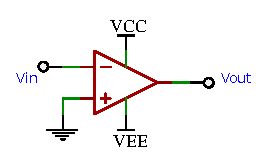
\includegraphics{circ_discr.pdf}
	\caption{Circuito Discriminatore}
	\label{f:discr}
\end{figure}

Si è montato il circuito come in \fig{discr}, inviando segnali sinusoidali in ingresso. La normale risposta del circuito può essere osservata in \fig{discr_normale}: di fatto, l'uscita è ad una tensione $\approx V_{CC} \approx \SI{15}{\V}$ quando l'ingresso è a tensione negativa, mentre è a $\approx V_{EE} \approx \SI{-15}{\V}$ quando l'ingresso è a tensione positiva. In realtà, il passaggio dell'output da alto a basso o viceversa avviene quando l'input attraversa una tensione leggermente diversa da 0: questa tensione di offset è stata misurata con l'oscilloscopio come la tensione dell'input nel momento in cui l'output inizia la discesa (o la salita), ottenendo il valore di \SI{31.8(34)}{\mV} (la cui incertezza è primariamente data dalla difficoltà nel riconoscere la contemporaneità delle due tensioni).
%TODO: magari vedere se dai dati presi per lo slewrate si può risalire al punto... è possibile i guess.

\begin{figure}[h]
	\centering
	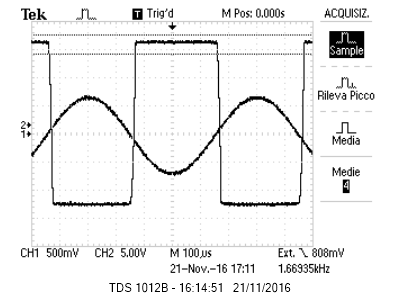
\includegraphics{risposta_normale_1.png}
	\caption{Risposta del discriminatore ad un segnale sinusoidale.}
	\label{f:discr_normale}
\end{figure}

Si è poi incrementata gradualmente la frequenza del segnale in ingresso, osservando la variazione del funzionamento del circuito ad alte frequenze.
Dapprima, e mantenendo l'ampiezza del segnale in ingresso a qualche volt, si osservano effetti legati allo slew rate finito dell'OpAmp: dal momento che il passaggio dell'output da $V_{CC}$ a $V_{EE}$ non può essere istantaneo, quando l'input ha un semiperiodo confrontabile col tempo richiesto per passare da +15 a \SI{-15}{\V} (che è costante) quest'ultimo diventa una parte sostanziale del periodo dell'output, che dunque si allontana dall'ideale onda quadra per avvicinarsi ad un'onda triangolare con fronti di salita e discesa aventi pendenza data dallo slew rate.
Si è dunque proceduto al fit dello slew rate dell'OpAmp. Acquisiti i dati attraverso l'oscilloscopio si è fittatta la retta affine (2 parametri). Per stimare l'errore di digitalizzazione si è fittato il segnale costante \SI{15}{\V} visibile all'inizio del grafico. Imponendo che il chi quadro fosse pari ai gradi di liberà di questo fit, si è così ottenuta una stima dell'errore di digitalizzazione dell'oscilloscopio.\footnote{Si sono ottenute in effetti tre stime, una massima (\SI{0.117}{V}), una media(\SI{0.124}{V}) e una minima(\SI{0.130}{V}), imponendo che il p-value fosse rispettivamente il $5\%$, $49\%$($\chi^2=\dof$) e $95\%$, non sono state attuate le solite procedure di propagazione lineare dell'errore dato che il $\chi^2$ è molto piccato. Si confronti il risultato con quanto atteso in modo banale dal numero di bin per divisione nella modalità grafica, ovvero 25 pt per divisione, dunque, a 5 V per divisione,  \SI{0.2}{V}} Come errore dei tempi si è scelto metà dell'intervallo di campionatura. Si sono dunque fittati i dati nella regione di interesse (fra $0 s$ e $\SI{-1.2e-6}{s}$) si sono ottenuti così i seguenti risultati	(dati e fit nel grafico \ref{f:SLW}):

$SR = \SI{18.771 \pm 0.015}{\mega\V\per\s}$\\
$q = \SI{-10.286 \pm 0.01}{\V}$\\
$\chi^2 = 537.07 (598 \dof, p = 0.97)$

\begin{figure}[h]
	\centering
	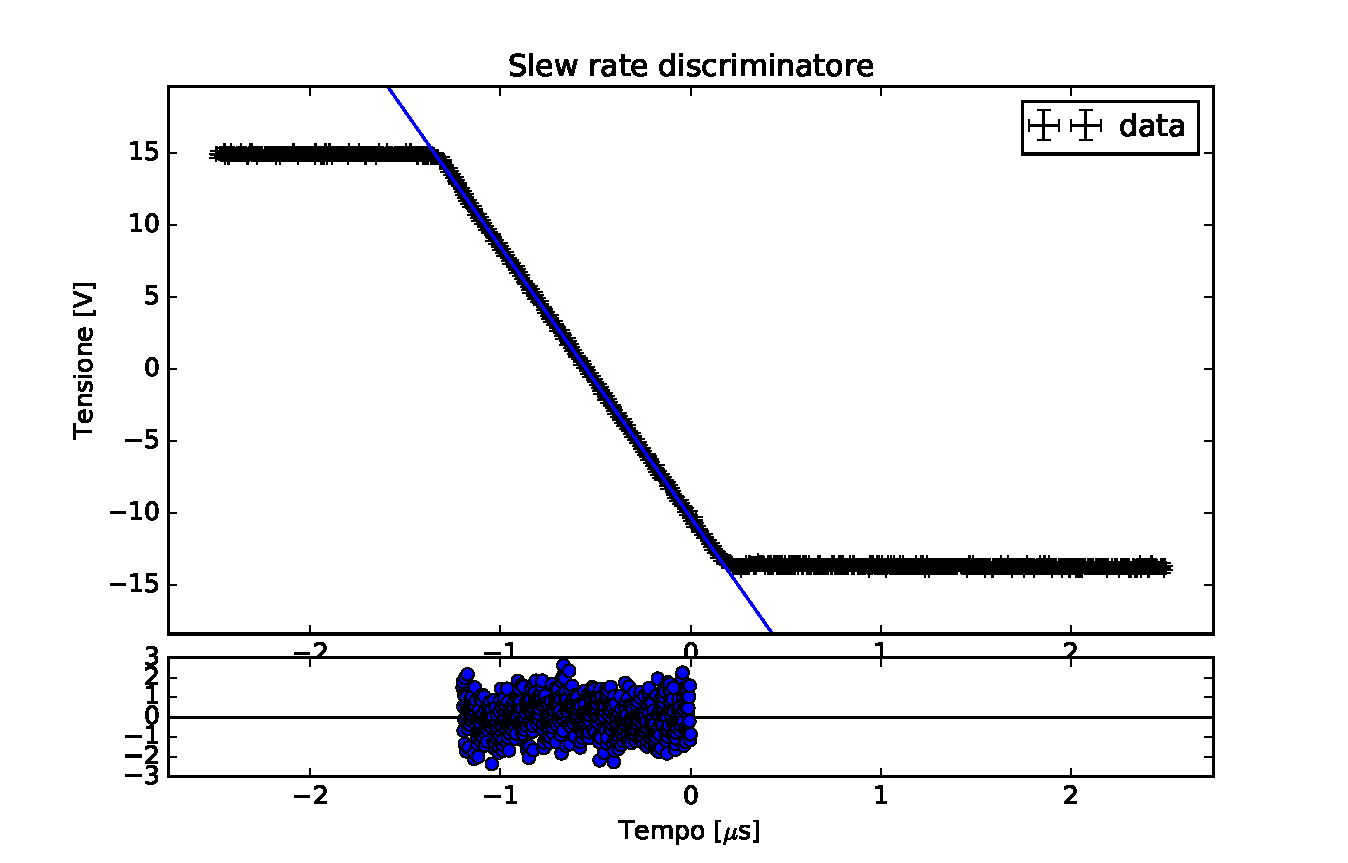
\includegraphics[scale=0.6]{slewfit.pdf}
	\caption{Fit dello slew-rate.}
	\label{f:SLW}
\end{figure}
Si vede come la procedura fornisca comunque un chi quadro non compatibile. Questo è però fisiologico in quanto la misura dell'errore fatta con la tecnica descritta ha essa stessa un errore, e questo errore si ripercuote sulla stima del $\chi^2$. Essendo la distribuzione del $\chi^2$ con 598 gradi di libertà abbastanza piccata, è possibile che variando l'errore nel errore sia possibile ottenere un p-value significativo. Non è stata però portata avanti questo tipo di analisi per \sbatta, si è solamente controllato che se si dovesse scegliere un chi-quadro della primo fit corrispondente a un p-value del 95\%, si otterrebbe un chi quadro per il secondo fit di $\chi^2 = 594.60 (598 \dof, p = 0.5316)$ (cosa che ci ha fatto propendere per questa spiegazione).



Passando a frequenze di qualche centinaio di \si{\kHz} e riducendo l'ampiezza dell'input si osserva un fenomeno particolare: poiché il guadagno dell'OpAmp a queste frequenze è significativamente inferiore, esso raggiunge la saturazione solo per ampiezze dell'input molto maggiori, dunque è apprezzabile per buona parte del periodo la risposta lineare dell'OpAmp, come si può vedere dalla \fig{gbw} (si nota inoltre la diversa relazione tra le fasi di ingresso e uscita rispetto alle basse frequenze, compatibile con il comportamento da circuito a un polo). Ci è però poco chiara la ragione dell'offset dell'output, che non sembra dovuto ad un possibile offset del generatore (poiché permane anche inserendo un condensatore tra questo e l'ingresso invertente dell'OpAmp) né riteniamo sia causato da una $V_{os} \neq 0$. %TODO possibilmente spiegare sta cosa ma nemmeno Forti l'ha capito quindi boh...

\begin{figure}[h]
	\centering
	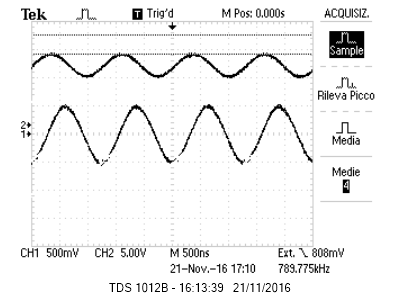
\includegraphics{gbw_1.png}
	\caption{Risposta del circuito ad alte frequenze e piccole ampiezze.}
	\label{f:gbw}
\end{figure}
